\section{Комбинаторика}

\subsection{Комбинаторные задачи}

Комбинаторные задачами называют задачи, в которых необходимо подсчитать, сколькими способами можно осуществить то или иное требование, выполнить какое-либо условие, сделать тот или иной выбор, то есть подсчет числа всевозможных комбинаций из элементов данного конечного множества при сделанных исходных предположениях.

\begin{example}
    У вас в темном чулане стоят банки с вареньем трех сортов: яблочное, сливовое и земляничное. Какое наименьшие количество банок вам надо взять, не глядя, чтобы среди них наверняка оказалось не менее девяти банок с вареньем одного сорта?

    Самый худший случай: \(8\) банок подряд с одним сортом варенья, затем \(8\) банок подряд с другим сортом, затем \(8\) банок подряд с третьим сортом:
    \[
        8 + 8 + 8 + 1 = 25.
    \]
\end{example}

\begin{example}
    Андрей, Борис, Виктор, Григорий и Дмитрий играли в шахматы. Каждый сыграл с каждым под одной партии. Сколько партий было сыграно?

    Решение для случая \(n = 5\):
    \[
        4 + 3 + 2 + 1 + 0 = 10.
    \]

    \begin{figure}[H]
        \centering
        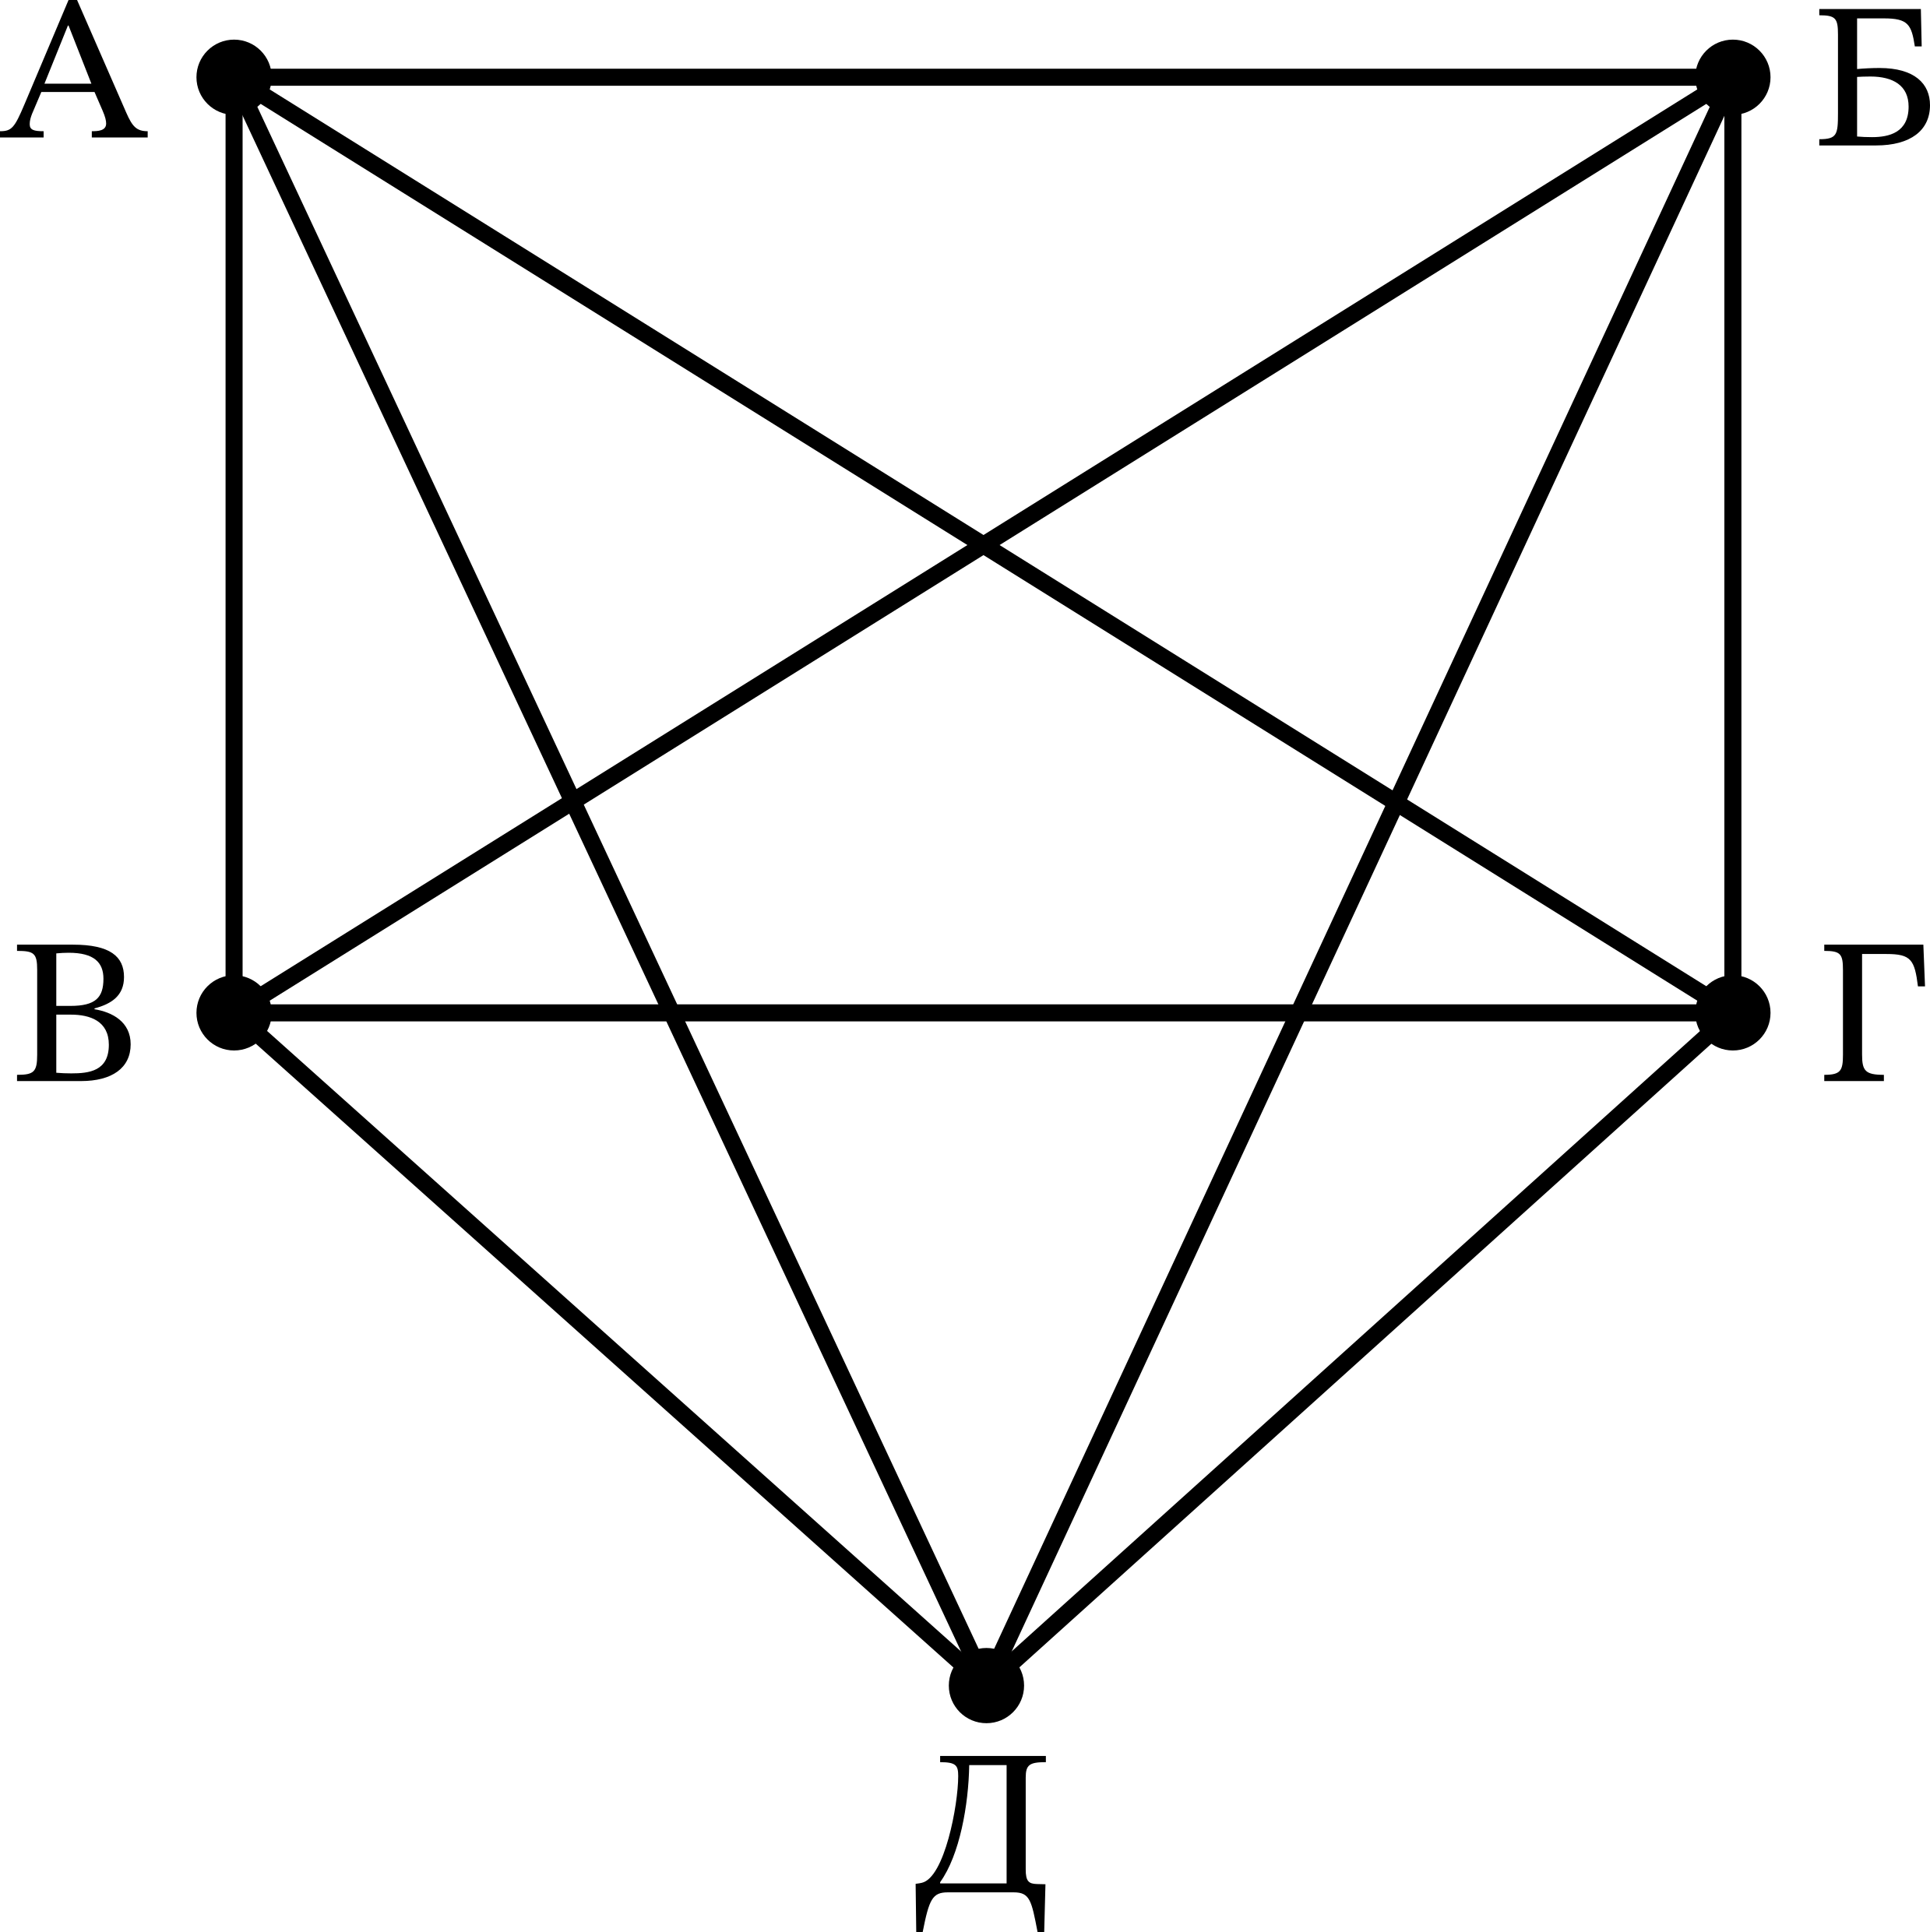
\includegraphics[width=0.4\textwidth]{images/graph-combinatorics.png}
        \caption{Решение с помощью графа}
    \end{figure}

    Решение для случая \(n\):
    \[
        (n - 1) + (n - 2) + \ldots + \ldots + 1 + 0 = \frac{n -1 + 0}{2} n = \frac{n(n - 1)}{2}.
    \]
\end{example}

\subsection{Правила суммы и произведения}

Если объект первого вида можно выбрать \(m\) способами, а объект второго вида -- \(n\) способами, то
\begin{itemize}
    \item один объект любого из этих видов можно выбрать \(m + n\) способами (правило суммы);
    \item пару объектов, один из которых первого вида, а другой -- второго вида, можно выбрать \(m \cdot n\) способами (правило произведения).
\end{itemize}

\begin{note*}
    Правила суммы и произведения справедливы для любого конечного числа видов объектов.
\end{note*}

\begin{example}
    В вазе лежит \(5\) яблок и \(3\) персика различных сортов. Сколькими способами можно выбрать один фрукт?

    По правилу суммы \(5 + 3 = 8\) вариантов.
\end{example}

\begin{example}
    Имеется \(2\) конверта: обычный и авиа, и \(3\) марки: прямоугольная, квадратная и треугольная. Сколькими способами можно выбрать конверт и марку, чтобы отправить письмо?

    По правилу произведения \(2 \cdot 3 = 6\) вариантов.
\end{example}

\begin{example}
    Сколько трехзначных чисел можно составить из \(1, 3, 5, 7\), используя в записи числа каждую из них не более одного раза?

    По правилу произведения \(4 \cdot 3 \cdot 2 = 24\) числа.
\end{example}

\begin{example}
    Сколько трехзначных чисел можно составить из \(1, 3, 5, 7\), используя в записи числа каждую из них любое число раз?

    По правилу произведения \(4 \cdot 4 \cdot 4 = 64\) числа.
\end{example}

\subsection{Схема выбора без возвращения}

\subsubsection{Перестановки}

Пусть имеется множество из \(n\) элементов. Каждая последовательность всех его элементов называется \textbf{перестановкой} из \(n\) элементов. Число всех перестановок из \(n\) элементов обозначается \(P_n\) и вычисляется по формуле:
\[
    P_n = n \cdot (n - 1) \cdot (n - 2) \cdot \ldots \cdot 1 = 1 \cdot 2 \cdot \ldots \cdot n = n!.
\]

\begin{example*}
    Имеется \(10\) различных книг. Сколько существует способов расставить их на одной книжной полке?

    Решение:
    \[
        n = 10
        \implies
        P_n = P_{10} = 10! = 3628800.
    \]
\end{example*}

\subsubsection{Размещения}

Пусть имеется множество из \(n\) элементов. \textbf{Упорядоченными подмножествами} этого множества называют различные последовательности, составленные из элементов подмножеств.

Каждое упорядоченное подмножество из \(k\) элементов множества из \(n\) элементов называется \textbf{размещением} из \(n\) элементов по \(k\) элементам. Число всех размещений из \(n\) элементов по \(k\) элементам обозначается \(A_n^k\) (читается <<\(A\) из \(n\) по \(k\)>>) и вычисляется по формуле:
\[
    A_n^k = n \cdot (n - 1) \cdot \ldots \cdot (n - k + 1) = \frac{n!}{(n - k)!}.
\]

\begin{example*}
    В турнире участвуют \(8\) спортсменов. Сколько можно сделать предсказаний относительно распределения первых трех мест?

    Решение:
    \[
        n = 8, k = 3
        \implies
        A_n^k = A_8^3 =
        \frac{8!}{(8 - 3)!} = 336.
    \]
\end{example*}

\begin{note*}
    Размещение \(A_n^n\) из \(n\) элементов по \(n\) элементам является перестановкой \(P_n\) из \(n\) элементов.
\end{note*}

\subsubsection{Сочетания}

Пусть имеется множество из \(n\) элементов. Каждое его подмножество из \(k\) элементов называется \textbf{сочетанием} из \(n\) элементов по \(k\) элементам. Таким образом, подмножества, отличающиеся друг от друга только порядком следования элементов, не считаются различными. Число всех сочетаний из \(n\) элементов по \(k\) элементам обозначается \(C_n^k\) (читается <<\(C\) из \(n\) по \(k\)>>) и вычисляется по формуле:
\[
    C_n^k = \frac{A_n^k}{k!} = \frac{n!}{k! (n - k)!}.
\]

\begin{example*}
    В группе \(25\) студентов. Надо выбрать трех человек, которые будут представлять группу на студенческой конференции. Сколькими способами можно осуществить этот выбор?

    Решение:
    \[
        n = 25, k = 3
        \implies
        C_n^k = C_{25}^3 = \frac{25!}{3! (25 - 3)!} = 2300.
    \]
\end{example*}

\subsection{Схема выбора с возвращением (с повторениями)}

\subsubsection{Перестановки с повторениями}

Пусть имеется мультимножество из \(n\) элементов \(k\) различных видов такое, что оно состоит из \(n_1\) элементов 1-го вида, \(n_2\) элементов 2-го вида, \ldots, \(n_k\) элементов \(k\)-го вида, причем \(n_1 + n_2 + \ldots + n_k = n\). Перестановки всех элементов такого мультимножества называются \textbf{перестановками с повторениями}.

\begin{theorem*}
    Число различных перестановок с повторениями равно
    \[
        P(n, n_1, \ldots, n_k) = \frac{n!}{n_1! \cdot \ldots \cdot n_k!}.
    \]
\end{theorem*}

\begin{example*}
    Определить, сколько различных слов можно составить из слова <<математика>>.

    В слове <<математика>> имеется 6 видов букв:
    \begin{multicols}{3}
        \begin{itemize}[label={}]
            \item букв <<м>> \(n_1 = 2\),
            \item букв <<е>> \(n_4 = 1\),
        \end{itemize}
        \begin{itemize}[label={}]
            \item букв <<а>> \(n_2 = 3\),
            \item букв <<и>> \(n_5 = 1\),
        \end{itemize}
        \begin{itemize}[label={}]
            \item букв <<т>> \(n_3 = 2\),
            \item букв <<к>> \(n_6 = 1\).
        \end{itemize}
    \end{multicols}
    Всего \(n = 2 + 3 + 2 + 1 + 1 + 1 = 10\) букв. Тогда из слова <<математика>> можно составить
    \[
        P(n, n_1, \ldots, n_6) = \frac{n!}{n_1! \cdot \ldots \cdot n_6!} = \frac{10!}{2! \cdot 3! \cdot 2! \cdot 1! \cdot 1! \cdot 1!} = 151200.
    \]
    различных слов.
\end{example*}

\subsubsection{Размещения с повторениями}

Пусть имеется множество из \(n\) элементов. Каждый кортеж длины \(k\), составленный из элементов данного \(n\)-элементного множества (элементы кортежа не обязательно должны быть различными), называется \textbf{размещением} из \(n\) элементов по \(k\) элементам \textbf{с повторениями}.

\begin{theorem*}
    Число всех размещений из \(n\) элементов по \(k\) элементам с повторениями равно:
    \[
        \bar{A}_n^k = \underbrace{n \cdot n \cdot \ldots \cdot n}_k = n^k.
    \]
\end{theorem*}

\begin{example*}
    Сколько пятизначных номеров можно составить из элементов множества \(\{1, 2, 3\}\)?

    Решение:
    \[
        n = 3, k = 5
        \implies
        \bar{A}_n^k = \bar{A}_3^5 = 3^5 = 243.
    \]
\end{example*}

\subsubsection{Сочетания с повторениями}

Пусть имеются элементы \(n\) различных видов. Из них составляется комбинация из \(k\) элементов такая, что порядок элементов в комбинации не важен, причем элементы одного вида могут повторяться. Такая комбинация называется \textbf{сочетанием с повторениями} из \(n\) элементов по \(k\) элементам.

\begin{theorem*}
    Число всех сочетаний с повторениями из \(n\) элементов по \(k\) элементам равно
    \[
        \bar{C}_n^k = C_{n + k - 1}^k.
    \]
\end{theorem*}

\begin{example*}
    В почтовом отделении продаются открытки пяти видов. Определить число способов покупки семи открыток.

    Решение:
    \[
        n = 5, k = 7
        \implies
        \bar{C}_n^k = \bar{C}_5^7 = C_{5 + 7 - 1}^7 = C_{11}^7 = 330.
    \]
\end{example*}

\subsection{Бином Ньютона}

Для произвольного положительного целого числа \(n\) справедлива следующая формула:
\[
    (a + b)^n =
    C_n^0 a^{n - 0} b^0 + C_n^1 a^{n - 1} b^1 + \ldots + C_n^n a^0 b^{n - 0} =
    \sum_{k = 0}^n C_n^k a^{n - k} b^k.
\]

Коэффициенты \(C_n^k\) называются \textbf{биномиальными коэффициентами} и вычисляются по формуле
\[
    C_n^k = \frac{n!}{k! (n - k)!}.
\]

\begin{example*}
    Определить разложение \((a + b)^n\) при \(n = 4\).

    Решение:
    \begin{gather*}
        (a + b)^4 =
        C_4^0 a^{4 - 0} b^0 + C_4^1 a^{4 - 1}b^1 + C_4^2 a^{4 - 2} b^2 + C_4^3 a^{4 - 3} b^3 + C_4^4 a^{4 - 4} b^4 = \\ =
        \frac{4!}{0! \cdot (4 - 0)!} a^4 + \frac{4!}{1! \cdot (4 - 1)!} a^3 b + \frac{4!}{2! \cdot (4 - 2)!} a^2 b^2 + \frac{4!}{3! \cdot (4 - 3)!} a b^3 + \\ + \frac{4!}{4! \cdot (4 - 4)!} b^4 =
        a^4 + 4 a^3 b + 6  a^2 b^2 + 4 a b^3 + b^4.
    \end{gather*}
\end{example*}

\subsection{Свойства биномиальных коэффициентов}

\begin{property}
    \[
        C_n^k = C_n^{n - k}.
    \]
    \begin{proof}
        \[
            C_n^{n - k} = \frac{n!}{(n - k)!(n - (n - k!))!} = \frac{n!}{(n - k)! k!} = \frac{n!}{k! (n - k)!} = C_n^k.
        \]
    \end{proof}
\end{property}

\begin{property}
    \[
        C_n^k = C_{n - 1}^k + C_{n - 1}^{k - 1}.
    \]
    \begin{proof}
        \begin{gather*}
            C_{n - 1}^k + C_{n - 1}^{k - 1} =
            \frac{(n - 1)!}{k! (n - 1 - k)!} + \frac{(n - 1)!}{(k - 1)! (n - 1 - k + 1)} = \\ =
            \frac{(n - 1)!}{(k - 1)! (n - k - 1)!} \Big( \frac{1}{k} + \frac{1}{n - k} \Big) =
            \frac{(n - 1)!}{(k - 1)! (n - k - 1)!} \cdot \frac{n - k + k}{k (n - k)} = \\ =
            \frac{(n - 1)! n}{(k - 1)! k (n - k - 1)! (n - k)} =
            \frac{n!}{k! (n - k)!} = C_n^k.
        \end{gather*}
    \end{proof}
\end{property}

\begin{property}
    \[
        C_n^i \cdot C_i^k = C_n^k \cdot C_{n - k}^{i - k}.
    \]
\end{property}

\begin{property}
    \[
        \sum_{k = 0}^n C_n^k = 2^n.
    \]
    \begin{proof}
        \[
            2^n = (1 + 1)^n = \sum_{k = 0}^n C_n^k \cdot 1^{n - k} \cdot 1^k = \sum_{k = 0}^n C_n^k.
        \]
    \end{proof}
\end{property}

\begin{property}
    \[
        \sum_{k = 0}^n (-1)^k C_n^k = 0.
    \]
\end{property}

\begin{property}
    \[
        \sum_{k = 0}^n k C_n^k = n 2^{n - 1}.
    \]
\end{property}

\begin{property}[тождество Коши]
    \[
        C_{m + n}^k = \sum_{i = 0}^k C_m^i C_n^{k - i}
    \]
\end{property}

\subsection{Треугольник Паскаля}

Рассмотрим следующий треугольник:

{
\renewcommand*{\arraystretch}{1.5}
\begin{longtable}{ccccccccc}
           &           &           &           & \(C_0^0\) &           &           &           &        \\
           &           &           & \(C_1^0\) &           & \(C_1^1\) &           &           &        \\
           &           & \(C_2^0\) &           & \(C_2^1\) &           & \(C_2^2\) &           &        \\
           & \(C_3^0\) &           & \(C_3^1\) &           & \(C_3^2\) &           & \(C_3^3\) &        \\
    \ldots &           & \ldots    &           & \ldots    &           & \ldots    &           & \ldots \\
\end{longtable}
}

Первая строка, состоящая из одного элемента, считается нулевой. Строка под номером \(n\) содержит биномиальные коэффициенты разложения \((a + b)^n\), то есть \(C_n^k\), где \(k\) пробегает значения от \(0\) до \(n\).

Элемент нулевой строки и боковые элементы треугольника равны единицам, а каждый внутренний элемент треугольника согласно свойству
\[
    C_n^k = C_{n - 1}^{k - 1} + C_{n - 1}^k
\]
равен сумме двух элементов, расположенных над ним. Таким образом, будем иметь:

{
\setlength{\tabcolsep}{3pt}
\begin{longtable}{ccccccccccccccccccccc}
           &       &        &       &        &        &        &        &        &         & \(1\)  &         &        &        &        &        &        &       &        &       &        \\
           &       &        &       &        &        &        &        &        & \(1\)   &        & \(1\)   &        &        &        &        &        &       &        &       &        \\
           &       &        &       &        &        &        &        & \(1\)  &         & \(2\)  &         & \(1\)  &        &        &        &        &       &        &       &        \\
           &       &        &       &        &        &        & \(1\)  &        & \(3\)   &        & \(3\)   &        & \(1\)  &        &        &        &       &        &       &        \\
           &       &        &       &        &        & \(1\)  &        & \(4\)  &         & \(6\)  &         & \(4\)  &        & \(1\)  &        &        &       &        &       &        \\
           &       &        &       &        & \(1\)  &        & \(5\)  &        & \(10\)  &        & \(10\)  &        & \(5\)  &        & \(1\)  &        &       &        &       &        \\
           &       &        &       & \(1\)  &        & \(6\)  &        & \(15\) &         & \(20\) &         & \(15\) &        & \(6\)  &        & \(1\)  &       &        &       &        \\
           &       &        & \(1\) &        & \(7\)  &        & \(21\) &        & \(35\)  &        & \(35\)  &        & \(21\) &        & \(7\)  &        & \(1\) &        &       &        \\
           &       & \(1\)  &       & \(8\)  &        & \(28\) &        & \(56\) &         & \(70\) &         & \(56\) &        & \(28\) &        & \(8\)  &       & \(1\)  &       &        \\
           & \(1\) &        & \(9\) &        & \(36\) &        & \(84\) &        & \(126\) &        & \(126\) &        & \(84\) &        & \(36\) &        & \(9\) &        & \(1\) &        \\
    \ldots &       & \ldots &       & \ldots &        & \ldots &        & \ldots &         & \ldots &         & \ldots &        & \ldots &        & \ldots &       & \ldots &       & \ldots \\
\end{longtable}
}

\begin{example}
    Используя треугольник Паскаля, найти \(C_5^2 + C_7^4 + C_9^6\).

    Решение:
    \[
        C_5^2 + C_7^4 + C_9^6 = 10 + 35 + 84 = 129.
    \]
\end{example}

\begin{example}
    Используя треугольник Паскаля, представить \((a + b)^7\) в виде многочлена:

    Решение:
    \[
        (a + b)^7 =
        a^7 + 7 a^6 b + 21 a^5 b^2 + 35 a^4 b^3 + 35 a^3 b^4 + 21 a^2 b^5 + 7 a b^6 + b^7.
    \]
\end{example}

\subsection{Полиномиальная формула}

Формула, обобщающая формулу бинома Ньютона, называется \textbf{полиномиальной}.

\begin{theorem*}
    Для любых натуральных чисел \(n\) и \(k\) и любых чисел \(a_1, \ldots, a_k\) справедлива формула
    \[
        (a_1 + \ldots + a_k)^n =
        \sum_{n_1 + \ldots + n_k = n} C(n, n_1, \ldots, n_k) \cdot a_1^{n_1} \cdot \ldots \cdot a_k^{n_k},
    \]
    где суммирование производится по всем решениям уравнения
    \[
        n_1 + n_2 + \ldots + n_k = n
    \]
    в неотрицательных целых числах.
\end{theorem*}

Коэффициенты данного разложения \(C(n, n_1, \ldots, n_k)\) называются \textbf{мультиномиальными коэффициентами} и вычисляются по формуле
\[
    C(n, n_1, \ldots, n_k) = \frac{n!}{n_1! \cdot \ldots \cdot n_k!}.
\]

Они совпадают с числом различных перестановок с повторениями:
\[
    P(n, n_1, \ldots, n_k) = \frac{n!}{n_1! \cdot \ldots \cdot n_k!}.
\]

\begin{example}
    Найти разложение степени \((a + b + c)^3\).

    Сначала определим число слагаемых в разложении:
    \[
        \bar{C}_3^3 = C_5^3 = \frac{5!}{3! \cdot 2!} = 10.
    \]
    \[
        (a + b + c)^3 = \sum_{n_1 + n_2 + n_3 = 3} C(3, n_1, n_2, n_3) a_1^{n_1} a_2^{n_2} a_3^{n_3},
    \]

    где
    \[
        C(3, n_1, n_2, n_3) = \frac{3!}{n_1! \cdot n_2! \cdot n_3!}.
    \]

    Возможно \(10\) решений уравнения \(n_1 + n_2 + n_3 = 3\) в целых числах:
    \begin{multicols}{2}
        \begin{enumerate}
            \item \(n_1 = 3\), \(n_2 = 0\), \(n_3 = 0\);
            \item \(n_1 = 2\), \(n_2 = 1\), \(n_3 = 0\);
            \item \(n_1 = 2\), \(n_2 = 0\), \(n_3 = 1\);
            \item \(n_1 = 1\), \(n_2 = 2\), \(n_3 = 0\);
            \item \(n_1 = 1\), \(n_2 = 1\), \(n_3 = 1\);
        \end{enumerate}
        \begin{enumerate}
            \setcounter{enumi}{5}
            \item \(n_1 = 1\), \(n_2 = 0\), \(n_3 = 2\);
            \item \(n_1 = 0\), \(n_2 = 3\), \(n_3 = 0\);
            \item \(n_1 = 0\), \(n_2 = 2\), \(n_3 = 1\);
            \item \(n_1 = 0\), \(n_2 = 1\), \(n_3 = 2\);
            \item \(n_1 = 0\), \(n_2 = 0\), \(n_3 = 3\).
        \end{enumerate}
    \end{multicols}

    \begin{gather*}
        (a + b + c)^3 =
        \frac{3!}{3! \cdot 0! \cdot 0!} a^3 b^0 c^0 + \frac{3!}{2! \cdot 1! \cdot 0!} a^2 b^1 c^0 + \frac{3!}{2! \cdot 0! \cdot 1!} a^2 b^0 c^1 + \\ + \frac{3!}{1! \cdot 2! \cdot 0!} a^1 b^2 c^0 + \frac{3!}{1! \cdot 0! \cdot 2!} a^1 b^0 c^2 + \frac{3!}{0! \cdot 2! \cdot 1!} a^0 b^2 c^1 + \frac{3!}{0! \cdot 1! \cdot 2!} a^0 b^1 c^2 + \\ + \frac{3!}{1! \cdot 1! \cdot 1!} a^1 b^1 c^1 + \frac{3!}{0! \cdot 3! \cdot 0!} a^0 b^3 c^0 + \frac{3!}{0! \cdot 0! \cdot 3!} a^0 b^0 c^3 = \\ =
        a^3 + 3 a^2 b + 3 a^2 c + 3 a b^2 + 3 a c^2 + 3 b^2 c + 3 b c^2 + 6 a b c + b^3 + c^3.
    \end{gather*}
\end{example}

\begin{example}
    В разложении многочлена \((1 + 2x^2 - 3x^4)^{10}\) найти коэффициент при \(x^8\).

    \begin{gather*}
        (1 + 2x^2 - 3x^4)^{10} =
        \sum_{n_1 + n_2 + n_3 = 10} \frac{10!}{n_1! \cdot n_2! \cdot n_3!} \cdot (1)^{n_1} \cdot (2x^2)^{n_2} \cdot (-3x^4)^{n_3} = \\ =
        \sum_{n_1 + n_2 + n_3 = 10} = \frac{10!}{n_1! \cdot n_2! \cdot n_3!} \cdot (2)^{n_2} \cdot (-3)^{n_3} \cdot x^{2n_2 + 4n_3}.
    \end{gather*}

    \[
        \begin{dcases}
            n_1 + n_2 + n_3 = 10 \\
            2n_2 + 4n_3 = 8.
        \end{dcases}
    \]

    \begin{enumerate}
        \item \(n_1 = 8\), \(n_2 = 0\), \(n_3 = 2\);
        \item \(n_1 = 7\), \(n_2 = 2\), \(n_3 = 1\);
        \item \(n_1 = 6\), \(n_2 = 4\), \(n_3 = 0\).
    \end{enumerate}

    Коэффициент при \(x^8\) вычисляется по формуле:
    \[
        \frac{10!}{n_1! \cdot n_2! \cdot n_3!} \cdot (2)^{n_2} \cdot (-3)^{n_3}.
    \]

    \begin{enumerate}
        \item \(n_1 = 8\), \(n_2 = 0\), \(n_3 = 2\):
              \[
                  \frac{10!}{8! \cdot 0! \cdot 2!} \cdot 2^0 \cdot (-3)^2 = 405;
              \]
        \item \(n_1 = 7\), \(n_2 = 2\), \(n_3 = 1\):
              \[
                  \frac{10!}{7! \cdot 2! \cdot 1!} \cdot 2^2 \cdot (-3)^1 = -4320;
              \]
        \item \(n_1 = 6\), \(n_2 = 4\), \(n_3 = 0\).
              \[
                  \frac{10!}{6! \cdot 4! \cdot 0!} \cdot 2^4 \cdot (-3)^0 = 3360.
              \]
    \end{enumerate}

    Таким образом, коэффициент при \(x^8\) будет равен:
    \[
        405 - 4320 + 3360 = -555.
    \]
\end{example}

\subsection{Схема упорядоченных разбиений}

Пусть имеется \(n\) различных шаров и \(k\) различных урн. Требуется разложить шары по урнам так, чтобы в \(i\)-й находилось \(m_i\) шаров, \(i = \overline{1, k}\), причем
\[
    m_1 + m_2 + \ldots + m_k = n.
\]
\[
    C(n, m_1, \ldots, m_k) = \frac{n!}{m_1! \cdot \ldots \cdot m_k!}.
\]

\begin{example}
    Известно, что принимая экзамен в группе из \(20\) человек, преподаватель поставил \(4\) <<пятерки>>, \(8\) <<четверок>>, \(5\) <<троек>> и \(3\) <<двойки>>. Сколько существует различных вариантов сдачи экзамена группой?

    Решение:
    \[
        C(20, 4, 8, 5, 3) = \frac{20!}{4! \cdot 8! \cdot 5! \cdot 3!} = 3491888400.
    \]
\end{example}

\subsection{Формула включений и исключений}

Формула, известная как \textbf{формула включений и исключений} позволяет вычислить мощность объединения множеств, если известны их мощности и мощности всех возможных пересечений.

\begin{theorem*}
    Пусть \(A_1, \ldots, A_n\) -- конечные множества. Тогда
    \begin{gather*}
        |A_1 \cup \ldots \cup A_n| =
        \sum_{1 \leq i_1 \leq n} |A_{i_1}| - \sum_{1 \leq i_1 < i_2 \leq n} |A_{i_1} \cap A_{i_2}| + \\ + \sum_{1 \leq i_1 < i_2 < i_3 \leq n} |A_{i_1} \cap A_{i_2} \cap A_{i_3}| - \ldots + (-1)^{n - 1} |A_1 \cap \ldots \cap A_n|.
    \end{gather*}
\end{theorem*}

\noindent Рассмотрим случай при \(n = 2\):
\[
    |A \cup B| = |A| + |B| - |A \cap B|.
\]

\noindent Рассмотрим случай при \(n = 3\):
\[
    |A \cup B \cup C| = |A| + |B| + |C| - |A \cap B|  - |A \cap B| - |B \cap C| + |A \cap B \cap C|.
\]

\noindent Рассмотрим случай при \(n = 4\):
\begin{gather*}
    |A \cup B \cup C \cup D| =
    |A| + |B| + |C| + |D| - |A \cap B| - |A \cap C| - |A \cap D| - \\ - |B \cap C| - |B \cap D| - |C \cap D| + |A \cap B \cap C| + |A \cap B \cap D| + \\ + |A \cap C \cap D| + |B \cap C \cap D| - |A \cap B \cap C \cap D|.
\end{gather*}

\begin{example}
    Сколько натуральных чисел в первой сотне, которые не делятся ни на \(2\), ни на \(5\), ни на \(7\)?
    \begin{gather*}
        A = \{ x \in \mathbb{N} \mid x \leq 100 \; \land \; x \divby 2 \},
        \qquad
        B = \{ x \in \mathbb{N} \mid x \leq 100 \; \land \; x \divby 5 \},
        \\
        C = \{ x \in \mathbb{N} \mid x \leq 100 \; \land \; x \divby 7 \}.
    \end{gather*}
    \[
        |A \cup B \cup C| = |A| + |B| + |C| + |A \cap B| - |A \cap C| - |B \cap C| + |A \cap B \cap C|.
    \]
    \[
        \overline{|A \cup B \cup C|} = |U| - |A \cup B \cup C|.
    \]
    \begin{gather*}
        |A| = \Bigg[ \frac{100}{2} \Bigg] = 50,
        \quad
        |B| = \Bigg[ \frac{100}{5} \Bigg] = 20,
        \quad
        |C| = \Bigg[ \frac{100}{7} \Bigg] = 14,
        \\
        |A \cap B| = \Bigg[ \frac{100}{\nok(2, 5)} \Bigg] = \Bigg[ \frac{100}{2 \cdot 5} \Bigg] = 10, \\
        |A \cap C| = \Bigg[ \frac{100}{\nok(2, 7)} \Bigg] = \Bigg[ \frac{100}{2 \cdot 7} \Bigg] = 7, \\
        |B \cap C| = \Bigg[ \frac{100}{\nok(5, 7)} \Bigg] = \Bigg[ \frac{100}{5 \cdot 7} \Bigg] = 2, \\
        |A \cap B \cap C| = \Bigg[ \frac{100}{\nok(2, 5, 7)} \Bigg] = \Bigg[ \frac{100}{2 \cdot 5 \cdot 7} \Bigg] = 1.
    \end{gather*}
    \[
        |A \cup B \cup C| = 50 + 20 + 14 - 10 - 7 - 2 + 1 = 66.
    \]
    \[
        \overline{|A \cup B \cup C|} = 100 - 66 = 34.
    \]

    \textbf{Ответ}: 34.
\end{example}

\begin{example}
    Человек хочет послать своему другу \(8\) различных фотографий. Сколькими способами он может это сделать, использовав \(5\) различных конвертов, если ни один конверт не должен быть пустым?

    Решение:
    \[
        5^8 - C_5^1 \cdot 4^8 + C_5^2 \cdot 3^8 - C_5^3 \cdot 2^8 + C_5^4 \cdot 1^8 = 126000.
    \]
\end{example}

\begin{example}
    Сколькими способами можно положить \(n\) различных предметов в \(m\) различных ящиков так, чтобы в каждом ящике лежал хотя бы один предмет?

    Решение:
    \[
        m^n - C_m^1 (m - 1)^n + C_m^2 (m - 2)^n - \ldots + (-1)^{m - 1} C_m^{m - 1} \cdot 1^n.
    \]
\end{example}

\begin{example}
    Сколькими способами можно положить \(n\) различных предметов в \(m\) \textbf{неразличимых} ящиков так, чтобы в каждом ящике лежат хотя бы один предмет?

    Решение:
    \[
        \frac{1}{m!} \Big( m^n - C_m^1 (m - 1)^n + C_m^2 (m - 2)^n - \ldots + (-1)^{m - 1} C_m^{m - 1} \cdot 1^n \Big).
    \]

    Полученная формула также называется \textbf{числом Стирлинга второго рода}.
\end{example}

\subsection{Задача о беспорядках}

\textbf{Беспорядком} называют перестановку \(n\) различных элементов, в которой ни один предмет не останется на своем первоначальном месте. Количество всех беспорядков обозначается \(D(n)\) и вычисляется по формуле:
\[
    D(n) = n! - C_n^1 (n - 1)! + C_n^2 (n - 2)! - \ldots + (-1)^n C_n^n (n - n)!.
\]

Учитывая, что
\[
    C_n^k \cdot (n - k)! = \frac{n!}{k!}
\]
формулу можно записать следующим образом:
\[
    D(n) =
    n! - \frac{n!}{1!} + \frac{n!}{2!} - \ldots + (-1)^n \frac{n!}{n!} =
    n! \Big( 1 - \frac{1}{1!} + \frac{1}{2!} - \ldots + (-1)^n \frac{1}{n!} \Big).
\]

Количество перестановок \(n\) различных предметов, при которых \(k\) предметов стоят на своих первоначальных местах, выражается числом
\[
    D(n, k) = C_n^k \cdot D(n - k).
\]

\subsection{Разбиения}

Пусть \(\{B_1, \ldots, B_k\}\) -- \textbf{разбиение} множества \(X\) из \(n\) элементов на \(k\) подмножеств:
\[
    B_i \subset X,
    \quad
    \bigcup_{i - 1}^k B_i = X,
    \quad
    B_i \neq \varnothing,
    \quad
    B_i \cap B_j = \varnothing \; \text{при} \; i \neq j.
\]
Подмножества \(B_i\) называются \textbf{блоками разбиения}.

\subsection{Число Стирлинга второго рода}

Число разбиений множества из \(n\) элементов на \(k\) непустых подмножеств (блоков) называется \textbf{числом Стирлинга второго рода} и обозначается \(S(n, k)\) или \(\displaystyle \begin{Bmatrix} n \\ k \end{Bmatrix} \) (читается <<\(k\) подмножеств из \(n\)>>). По определению полагают:
\begin{gather*}
    S(n, n) = 1,
    \quad
    S(n, 0) = 0 \; \text{при} \; n > 0,
    \\
    S(0, 0) = 1,
    \quad
    S(n, k) = 0 \; \text{при} \; k > n.
\end{gather*}

\textbf{Рекуррентная формула}:
\[
    S(n, k) = S(n - 1, k -1) + k \cdot S(n - 1, k) \; \text{для} \; 0 < k < n.
\]

\textbf{Явная формула}:
\[
    S(n, k) = \frac{1}{k!} \sum_{i = 0}^k (-1)^{k + i} C_k^i \cdot i^n.
\]

Число размещений \(n\) предметов по \(k\) ящикам так, чтобы все ящики были заняты, вычисляется по формуле
\[
    k! \cdot S(n, k).
\]

\begin{example}
    Найти число разбиений четырехэлементного множества на две части. Пусть таким четырехэлементным множеством будет множество \(\{1, 2, 3, 4\}\). Тогда получим следующие разбиения:
    \begin{gather*}
        \{1, 2, 3\} \cup \{4\},
        \quad
        \{1, 2, 4\} \cup \{3\},
        \quad
        \{1, 3, 4\} \cup \{2\},
        \quad
        \{2, 3, 4\} \cup \{1\}, \\
        \quad
        \{1, 2\} \cup \{3, 4\},
        \quad
        \{1, 3\} \cup \{2, 4\},
        \quad
        \{1, 4\} \cup \{2, 3\}.
    \end{gather*}

    Итого получаем, что \(S(4, 2) = 7\). Получим тот же результат с помощью формулы:
    \[
        S(4, 2) =
        \frac{1}{2!} \Big( (-1)^2 C_2^0 0^4 + (-1)^3 C_2^1 1^4 + (-1)^4 C_2^2 2^4 \Big) =
        \frac{14}{2} = 7.
    \]
\end{example}

\begin{example}
    Найти число разбиений пятиэлементного множества на три части.

    Решение:
    \begin{gather*}
        S(5, 3) = \frac{1}{3!} \Big( (-1)^3 C_3^0 0^5 + (-1)^4 C_3^1 1^5 + (-1)^5 C_3^2 2^5 + (-1)^6 C_3^3 3^5 \Big) = \\
        = \frac{150}{6} = 25.
    \end{gather*}
\end{example}

\subsection{Число Белла}

Число всех разбиений множества из \(n\) элементов называется \textbf{числом Белла} и обозначается \(B(n)\):
\[
    B(n) = \sum_{k = 1}^n S(n, k),
    \qquad
    B(0) = 1.
\]

\begin{theorem*}
    Числа Белла удовлетворяют следующему рекуррентному соотношению:
    \[
        B(n + 1) = \sum_{k = 0}^n C_n^k B(k).
    \]
\end{theorem*}

\begin{example}
    Найти число всех возможных разбиений трехэлементного множества.

    Решение c помощью числа Белла:
    \begin{gather*}
        B(3) =
        \sum_{k = 1}^3 S(3, k) =
        S(3, 1) + S(3, 2) + S(3, 3) = \\ =
        1 + \frac{1}{2!} \Big( (-1)^2 C_2^0 0^3 + (-1)^3 C_2^1 1^3 + (-1)^4 C_2^2 2^3 \Big) + 1 =
        1 + \frac{6}{2} + 1 = 5.
    \end{gather*}

    Это легко проверить на примере множества \(\{a, b, c\}\):
    \begin{gather*}
        \{\{a\}, \{b\}, \{c\}\},
        \quad
        \{\{a, b\}, \{c\}\},
        \quad
        \{\{a, c\}, \{b\}\}, \\
        \quad
        \{\{a\}, \{b, c\}\},
        \quad
        \{\{a, b, c\}\}.
    \end{gather*}
\end{example}

\begin{example}
    Найти \(B(4)\), используя рекуррентное соотношение.

    Решение:
    \begin{gather*}
        B(4) =
        \sum_{k = 0}^3 C_3^k B(k) =
        C_3^0 B(0) + C_3^1 B(1) + C_3^2 B(2) + C_3^3 B(3) = \\ =
        1 \cdot 1 + 3 \cdot 1 + 3 \cdot 2 + 1 \cdot 5 =
        15.
    \end{gather*}
\end{example}

\subsection{Треугольник Белла}

\noindent Принцип построения треугольника Белла:
\begin{itemize}
    \item первая строка содержит \(1\);
    \item каждая следующая строка начинается числом, стоящим в конце предыдущей строки;
    \item каждое следующее число в строке равно сумме чисел, стоящих слева и сверху от него;
    \item числа Белла образуют последние числа в строках.
\end{itemize}

{
\renewcommand*{\arraystretch}{1.5}
\setlength{\tabcolsep}{1pt}
\begin{longtable}{ccccccccccccccccc}
               &         &            &          &            &          &            &          & \(1\)      &          &            &          &            &          &            &          &            \\
               &         &            &          &            &          &            & \(1\)    &            & \(2\)    &            &          &            &          &            &          &            \\
               &         &            &          &            &          & \(2\)      &          & \(3\)      &          & \(5\)      &          &            &          &            &          &            \\
               &         &            &          &            & \(5\)    &            & \(7\)    &            & \(10\)   &            & \(15\)   &            &          &            &          &            \\
               &         &            &          & \(15\)     &          & \(20\)     &          & \(27\)     &          & \(37\)     &          & \(52\)     &          &            &          &            \\
               &         &            & \(52\)   &            & \(67\)   &            & \(87\)   &            & \(114\)  &            & \(151\)  &            & \(203\)  &            &          &            \\
               &         & \(203\)    &          & \(255\)    &          & \(322\)    &          & \(409\)    &          & \(523\)    &          & \(674\)    &          & \(877\)    &          &            \\
               & \(877\) &            & \(1080\) &            & \(1335\) &            & \(1657\) &            & \(2066\) &            & \(2589\) &            & \(3263\) &            & \(4140\) &            \\
    \(\ldots\) &         & \(\ldots\) &          & \(\ldots\) &          & \(\ldots\) &          & \(\ldots\) &          & \(\ldots\) &          & \(\ldots\) &          & \(\ldots\) &          & \(\ldots\) \\
\end{longtable}
}

{
\renewcommand*{\arraystretch}{1.5}
\setlength{\tabcolsep}{10pt}
\begin{longtable}{|c|c|c|c|c|c|c|c|c|c|}
    \hline
    \(n\)    & \(0\) & \(1\) & \(2\) & \(3\) & \(4\)  & \(5\)  & \(6\)   & \(7\)   & \(8\)    \\
    \hline
    \(B(n)\) & \(1\) & \(1\) & \(2\) & \(5\) & \(15\) & \(52\) & \(203\) & \(877\) & \(4140\) \\
    \hline
\end{longtable}
}

\subsection{Числа Фибоначчи}

Числа Фибоначчи \(F(n)\) определяются следующим образом:
\[
    F(0) = 1,
    \quad
    F(1) = 1,
    \quad
    \forall n \; \geq 0 \; F(n + 2) = F(n + 1) + F(n).
\]

Последовательность Фибоначчи имеет вид:
\[
    1, 1, 2, 3, 5, 8, 13, 21, 34, 55, 89, 144, 233, \ldots.
\]

\(F(n + 2) - F(n + 1) - F(n) = 0\) представляет собой линейное однородное разностное уравнение второго порядка, его характеристическое уравнение имеет вид:
\[
    \lambda^2 - \lambda - 1 = 0
    \implies
    \lambda_{1, 2} = \frac{1 \pm \sqrt{5}}{2}.
\]

Положительный корень этого уравнения обозначается греческой буквой \(\Phi\) (фи):
\[
    \Phi = \frac{1 + \sqrt{5}}{2} \approx 1.618
\]
и называется <<Золотым сечением>>.

\textbf{Золотое сечение} -- это такое пропорциональное деление отрезка на неравные части, при котором весь отрезок так относится к большей части, как сама большая часть относится к меньшей (отношение меньшей части к большей равно отношению большей части к длине всего отрезка)
\[
    \lim_{n \to \infty} \frac{F(n + 1)}{F(n)} = \Phi.
\]

Формула для вычисления чисел Фибоначчи имеет вид:
\[
    F(n) = \frac{1}{\sqrt{5}} \Bigg( \bigg(\frac{1 + \sqrt{5}}{2} \bigg)^{n + 1} - \bigg( \frac{1 - \sqrt{5}}{2} \bigg)^{n + 1} \Bigg).
\]

\subsection{Числа Каталана}

Числа Каталана используются при решении различных комбинаторных задач, обозначаются \(C(n)\) и определяются следующим рекуррентным соотношением:
\[
    C(0) = 1,
    \qquad
    C(n) = \sum_{k = 0}^{n - 1} C(k) \cdot C(n - k - 1).
\]

Числа Каталана выражаются через биномиальные коэффициенты:
\[
    C(n) = \frac{C_{2n}^n}{n + 1} = \frac{1}{n + 1} C_{2n}^n
\]

Числа Каталана встречаются в большом количестве задач комбинаторики. Так, например, \(n\)-е число Каталана -- это:
\begin{itemize}
    \item количество корректных скобочных последовательностей, состоящих из \(n\) открывающих и \(n\) закрывающих скобок;
    \item количество корневых бинарных деревьев с \(n + 1\) листьями (вершины не пронумерованы);
    \item количество триангуляций выпуклого \(n + 2\)-угольника;
    \item количество способов соединить \(2n\) точек на окружности \(n\) непересекающимся хордами.
\end{itemize}
